\documentclass{standalone}
\usepackage{tikz}

\usetikzlibrary{calc}

\begin{document}

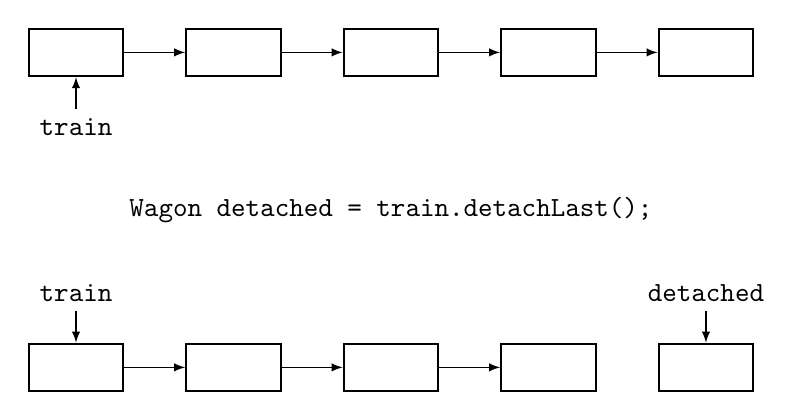
\begin{tikzpicture}[wagon/.style={minimum width=1.2cm,minimum height=0.6cm,draw,black,thick},
                    link/.style={-latex,thin},
                    address/.style={font=\tiny,circle,thin,fill=white}]

  \foreach[count=\i] \c in {20,30,25,55,5} {
    \pgfmathparse{(\i-1)*2}\let\x\pgfmathresult
    \node[wagon] (w\i) at (\x,0) {};
  }
  \foreach \i in {1,2,3,4} {
    \pgfmathparse{int(\i+1)}\let\j\pgfmathresult
    \draw[link] (w\i.east) -- (w\j.west);
  }

  \begin{scope}[yshift=-4cm]
    \foreach[count=\i] \c in {20,30,25,55,5} {
      \pgfmathparse{(\i-1)*2}\let\x\pgfmathresult
      \node[wagon] (ww\i) at (\x,0) {};
    }
    \foreach \i in {1,2,3} {
      \pgfmathparse{int(\i+1)}\let\j\pgfmathresult
      \draw[link] (ww\i.east) -- (ww\j.west);
    }
  \end{scope}

  \node[anchor=north] (var) at ($ (w1.south) + (0,-.4) $) {\tt train};
  \draw[-latex] (var.north) -- (w1.south);

  \node[anchor=south] (var) at ($ (ww1.north) + (0,.4) $) {\tt train};
  \draw[-latex] (var.south) -- (ww1.north);

  \node[anchor=south] (var2) at ($ (ww5.north) + (0,.4) $) {\tt detached};
  \draw[-latex] (var2.south) -- (ww5.north);

  \node at ($ (ww1.north west) ! .5 ! (w5.south east) $) {\tt Wagon detached = train.detachLast();};
\end{tikzpicture}

\end{document}